\documentclass[a4paper,10pt]{article}
\usepackage[pdftex]{color,graphicx}
\usepackage[pdftex, bookmarks, colorlinks]{hyperref}
\usepackage{longtable}
\addtolength{\textheight}{2cm}
\addtolength{\textwidth}{2cm}
\addtolength{\hoffset}{-1cm}
\addtolength{\voffset}{-3cm}

%opening
\title{GWA Sections}
\author{Yu Huang}

\begin{document}

\maketitle

\begin{abstract}

\end{abstract}

\tableofcontents


\section{Over-representation of Priori Candidate Gene List}
For several phenotypes, we were able to collect a priori candidate gene list from literature/TAIR website. These candidate gene lists allow us to check whether the results by different methods make biological sense apart from statistical inspection. We also use some GeneOntology categories that meet certain criteria, (like each category has to cover 100 genes, etc), as another kind of candidate gene lists.

One tricky point is how to associate genes to individual SNPs. First question how far away the gene should be to be counted as associated with the SNP. Second question is whether to take all genes within a certain distance or just the closest gene. The over-representation tests will calculated under different parameters.

\subsection{Rank sum test}

First test is a rank sum test, Mann-Whitney test, that compares the p-values of candidate genes versus those of non-candidate genes. Figure ~\ref{f1} shows one result. Correpondance between phenotype and candidate gene list is not very specific. There are several possible reasons. First, taking maximum pvalue out of several SNPs that are associated with a gene is gonna cause a bias for genes with lots of markers. Second, the priori candidate gene list contains different types of genes, not all of them are directly related to the specific phenotype, Figure~\ref{f2}. Results from different phenotypes are matching those different types. This will become clear in Figure~\ref{f6}, showing the number of overlapping top ranked genes among results from different phenotypes.

\begin{figure}
  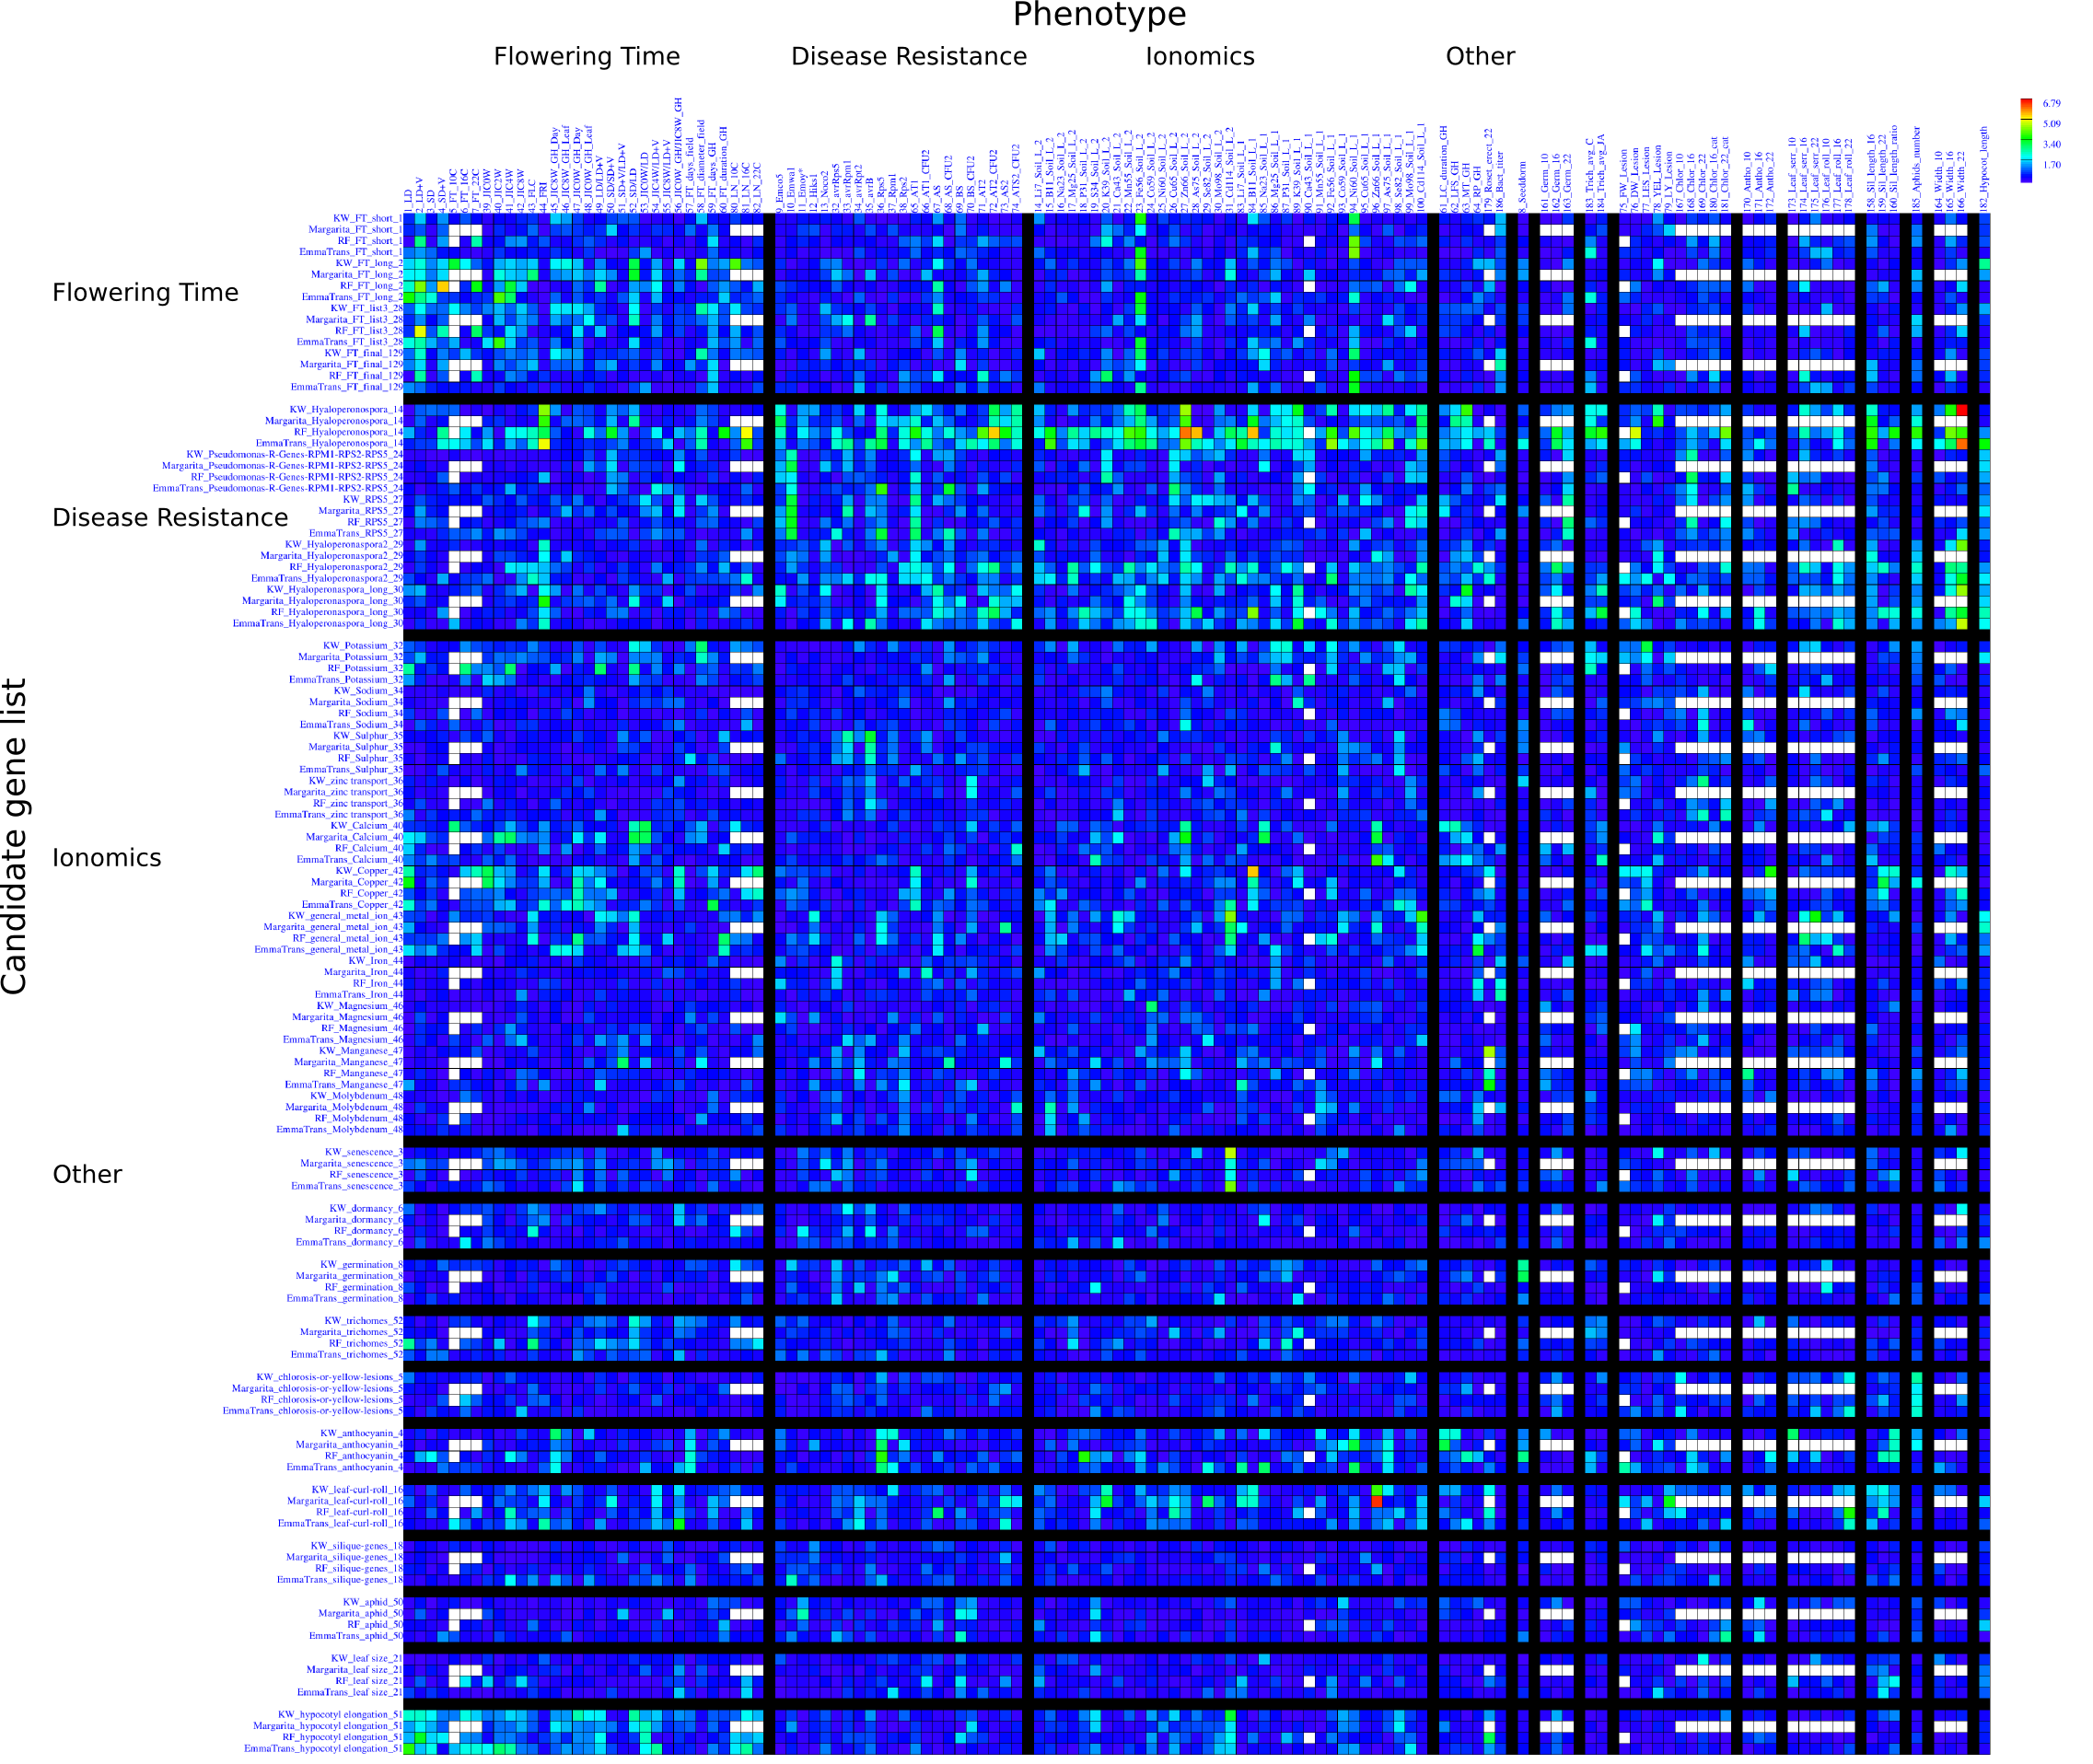
\includegraphics[width=0.9\textwidth]{figures/rank_sum_test_call_method_17_m20000_inkscape.png}
  \caption{Significance level of rank sum test results. All genes within 20,000 bp from the SNP are assigned with that SNP's pvalue. In case of one gene having multiple pvalues from different SNPs, the maximum will be taken as that gene's pvalue. Rows are different types of candidate gene list with different methods. Columns are different phenotypes. Black bar separates similar groups of phenotypes.}\label{f1}
\end{figure}

\begin{figure}
  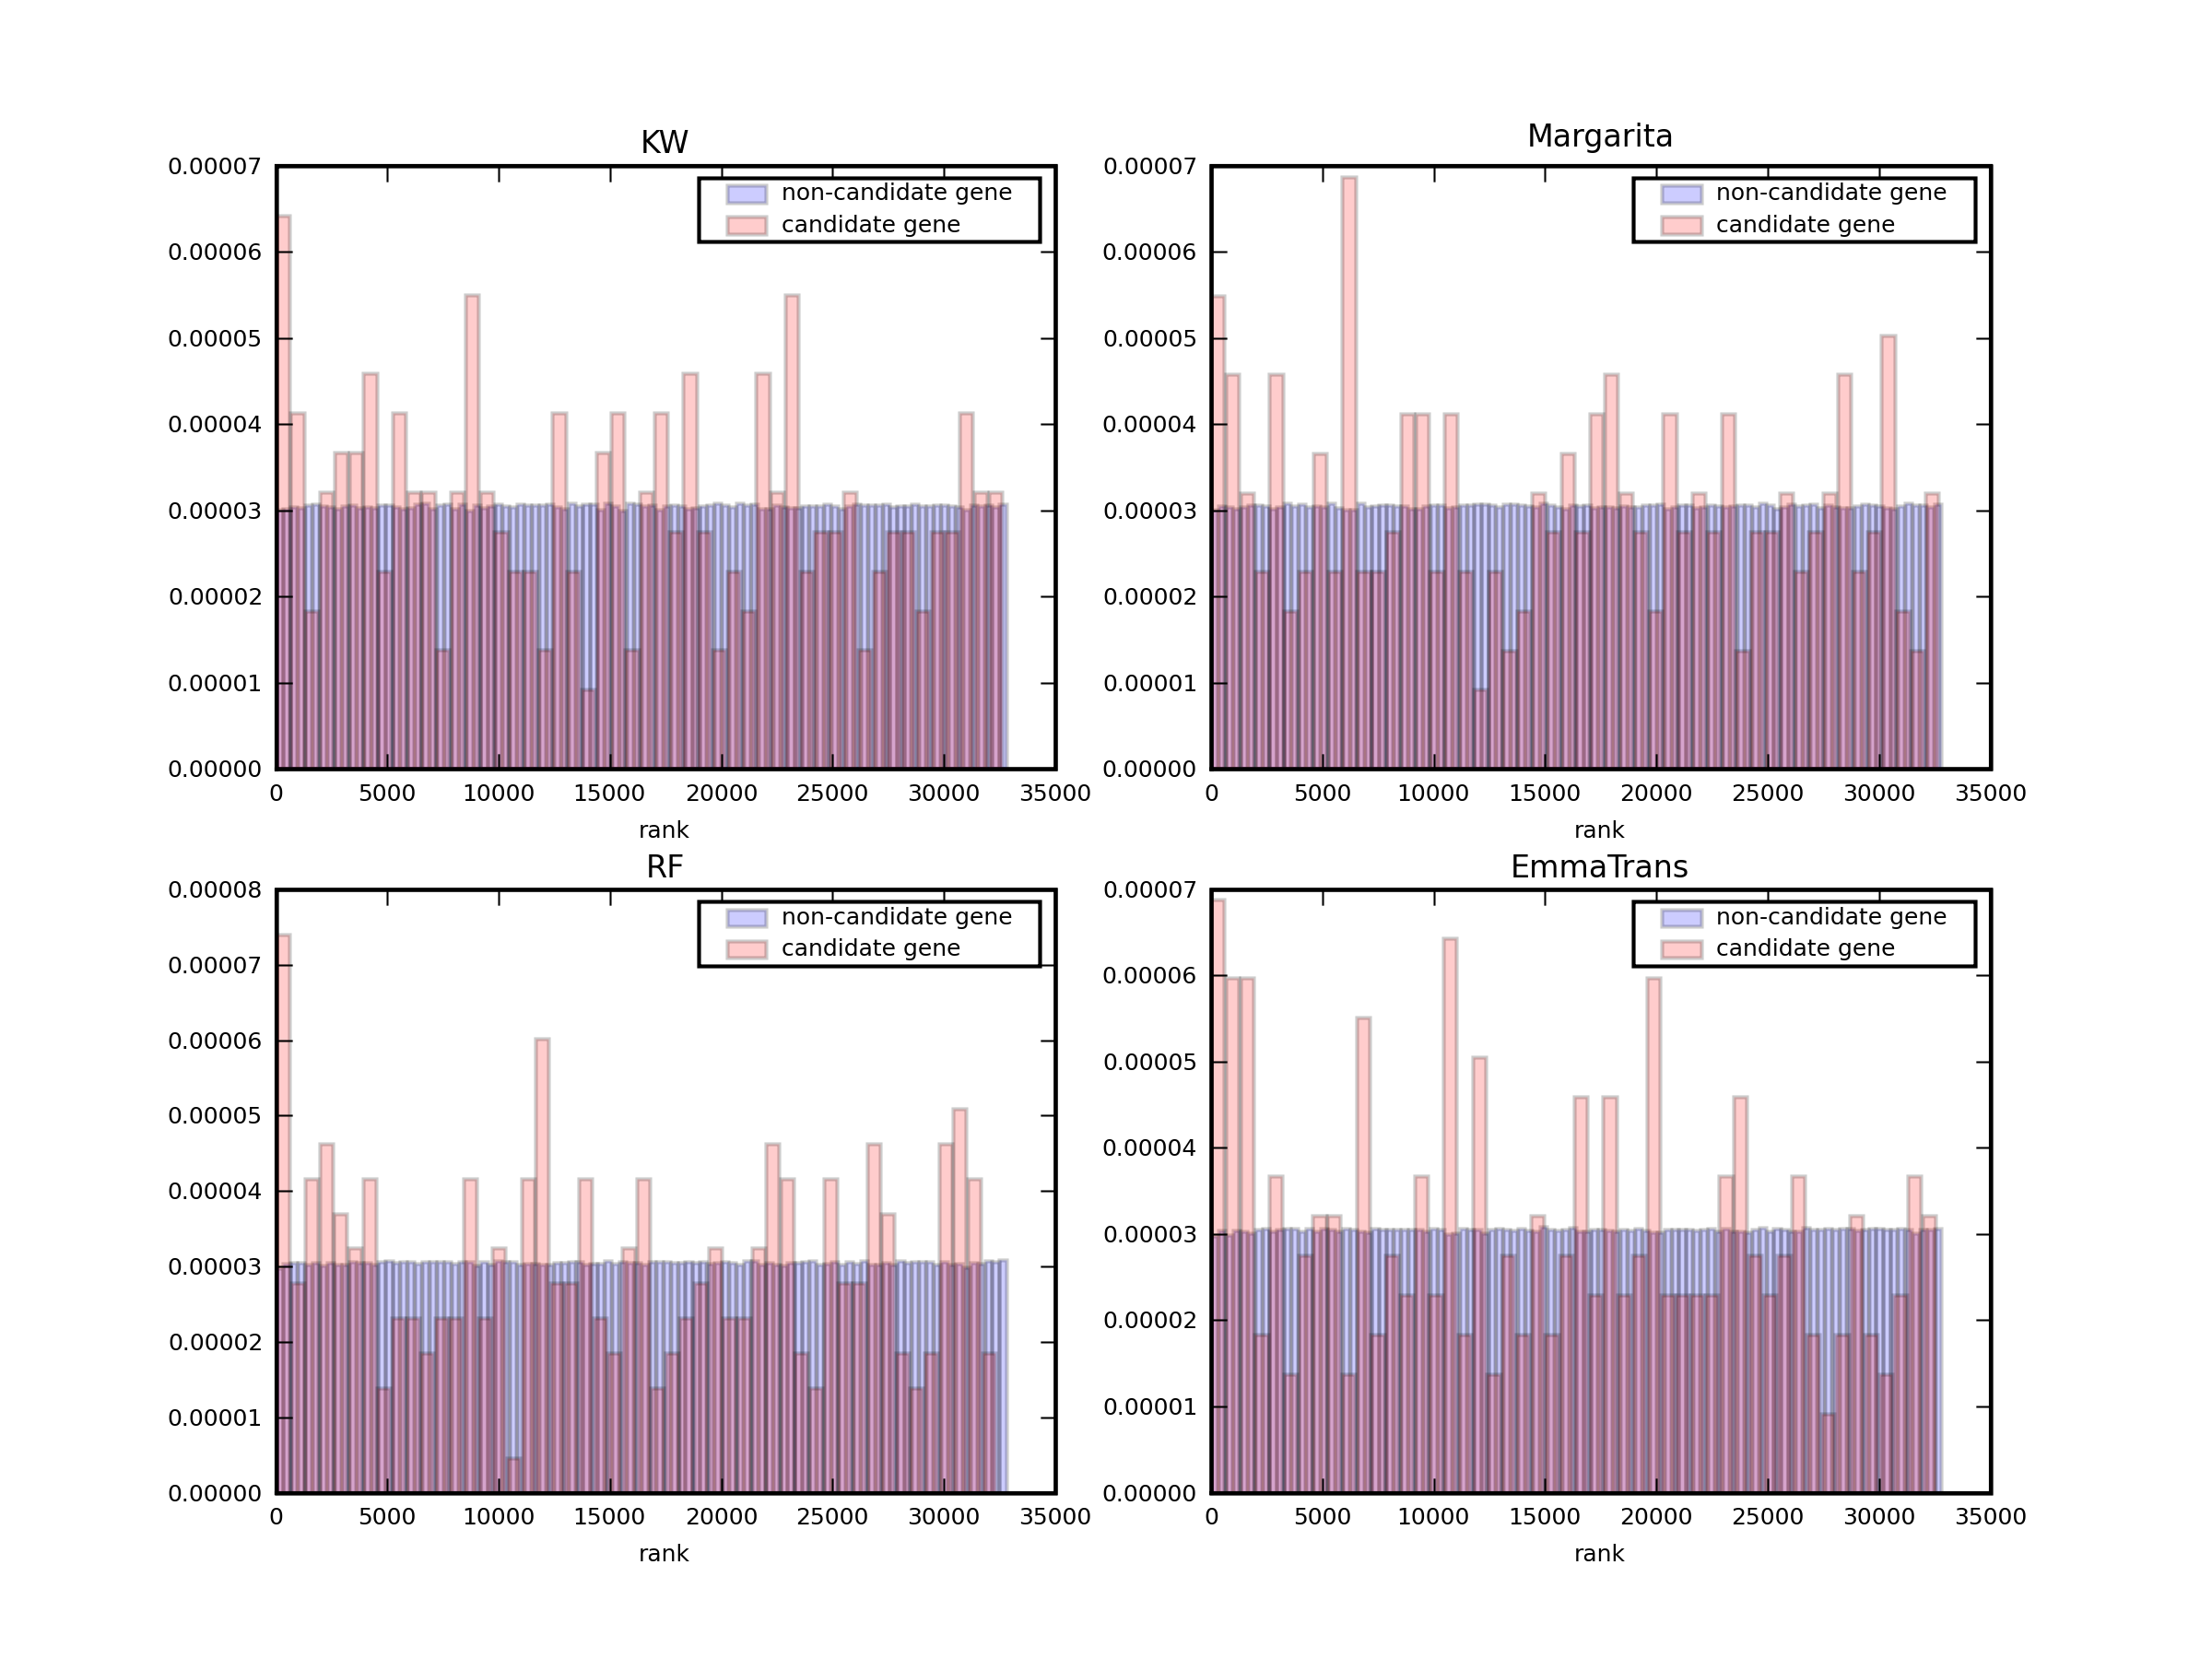
\includegraphics[width=0.9\textwidth]{figures/1_LD_28_FT_list3_rank.png}
  \caption{Histogram of ranks of candidate genes versus non-candidate genes in all 4 methods. The phentoype is long-day flowering time without vernalization. Clearly, there are candidate genes ranked pretty low.}\label{f2}
\end{figure}

\subsection{Hypergeometric test}

Second test we apply is the hypergeometric test to check the enrichment of candidate genes among the top-ranked genes. Figure ~\ref{f3} shows a result with maximum gene-association distance=20kb. The correpondance between phenotype and candidate gene list is more specific than the rank sum test results.  Figure~\ref{f4} is same as Figure~\ref{f3} except only genes closest to a SNP are assigned with  that SNP's pvalue. Signal is noiser. 20kb appears to be the optimum distance to associate genes to a SNP because it shows the cleanest picture (data not shown). The number of top-ranked genes is more flexible. Number up to 1000 could still give good results, Figure~\ref{f5}.

\begin{figure}
  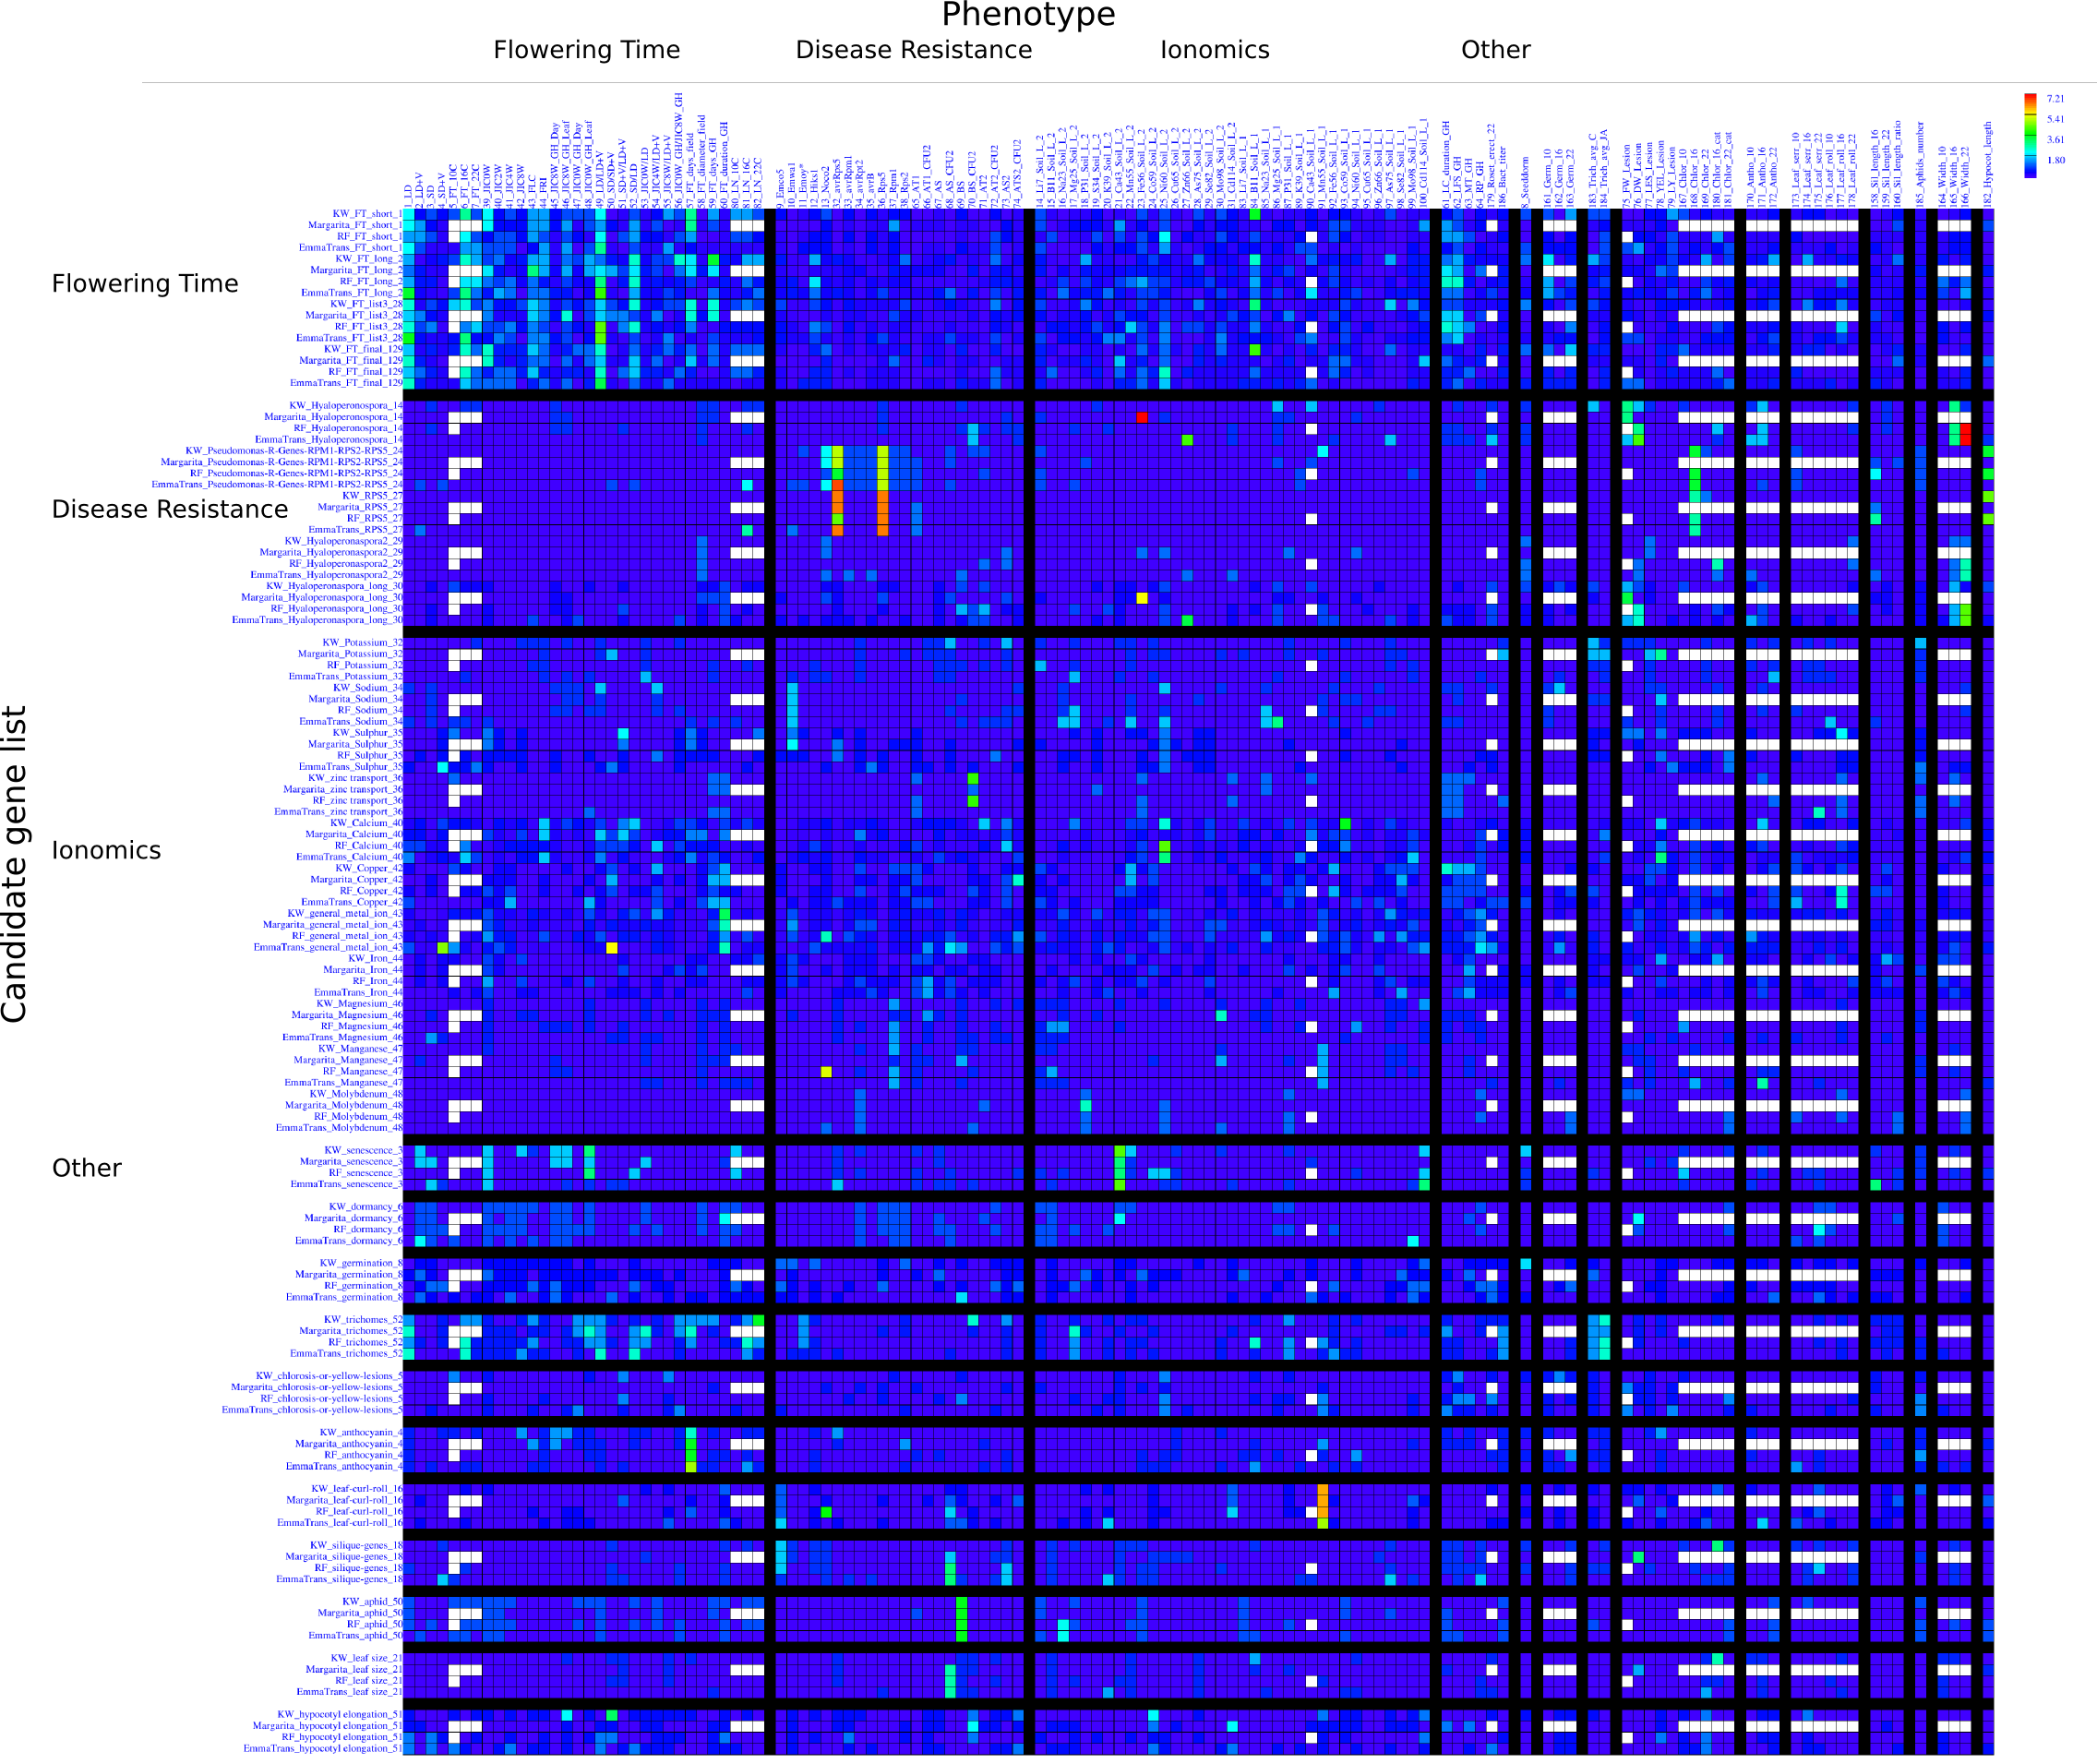
\includegraphics[width=1\textwidth]{figures/top_snp_test_call_method_17_f200_m20000_inkscape.png}
  \caption{Enrichment of candidate genes among top 200 genes. All genes within 20,000 bp from the SNP are assigned with that SNP's pvalue. In case of one gene having multiple pvalues from different SNPs, the maximum will be taken as that gene's pvalue. Rows are different types of candidate gene list with different methods. Columns are different phenotypes. Black bar separates similar groups of phenotypes.}\label{f3}
\end{figure}

\begin{figure}
  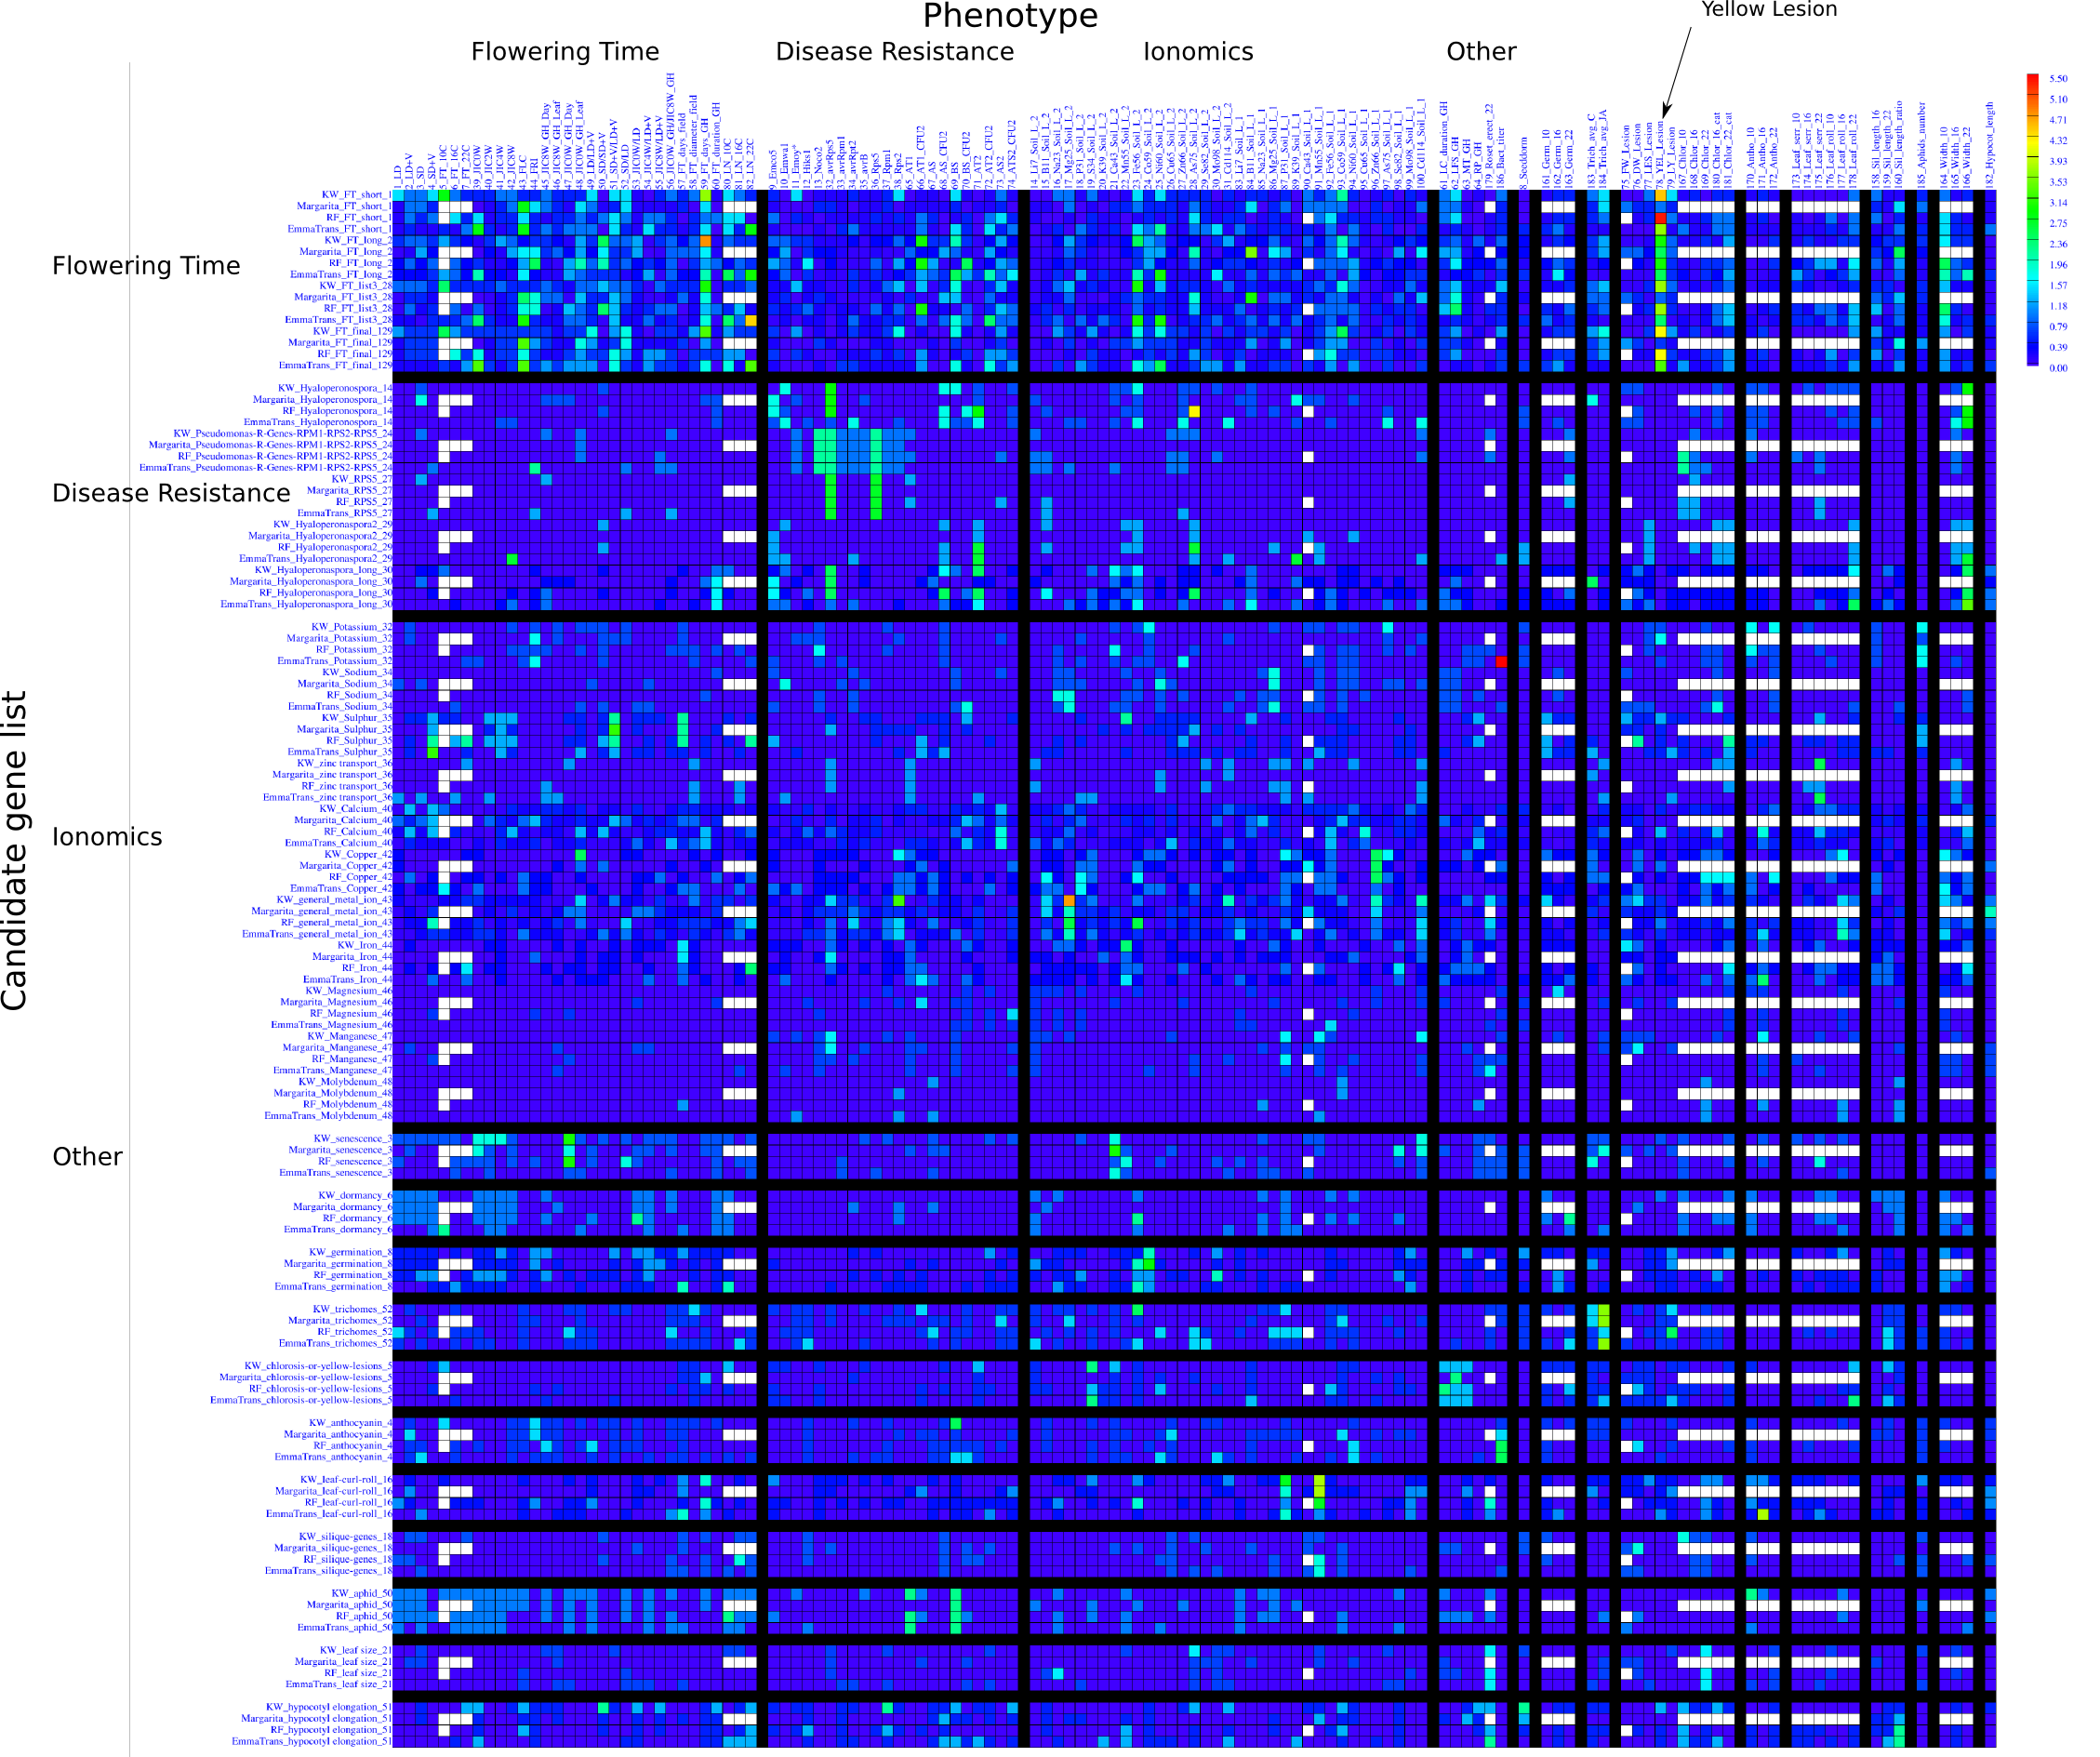
\includegraphics[width=1\textwidth]{figures/top_snp_test_call_method_17_f200_m20000_g_inkscape.png}
  \caption{Enrichment of candidate genes among top 200 genes. \textbf{Only closest genes} within 20,000 bp from the SNP are assigned with that SNP's pvalue. In case of one gene having multiple pvalues from different SNPs, the maximum will be taken as that gene's pvalue. Rows are different types of candidate gene list with different methods. Columns are different phenotypes. Black bar separates similar groups of phenotypes. Signal is noisier than Figure~\ref{f3}. Phenotype called 'Yellow Lesion' shows strong enrichment of flowering time genes.}\label{f4}
\end{figure}

\begin{figure}
  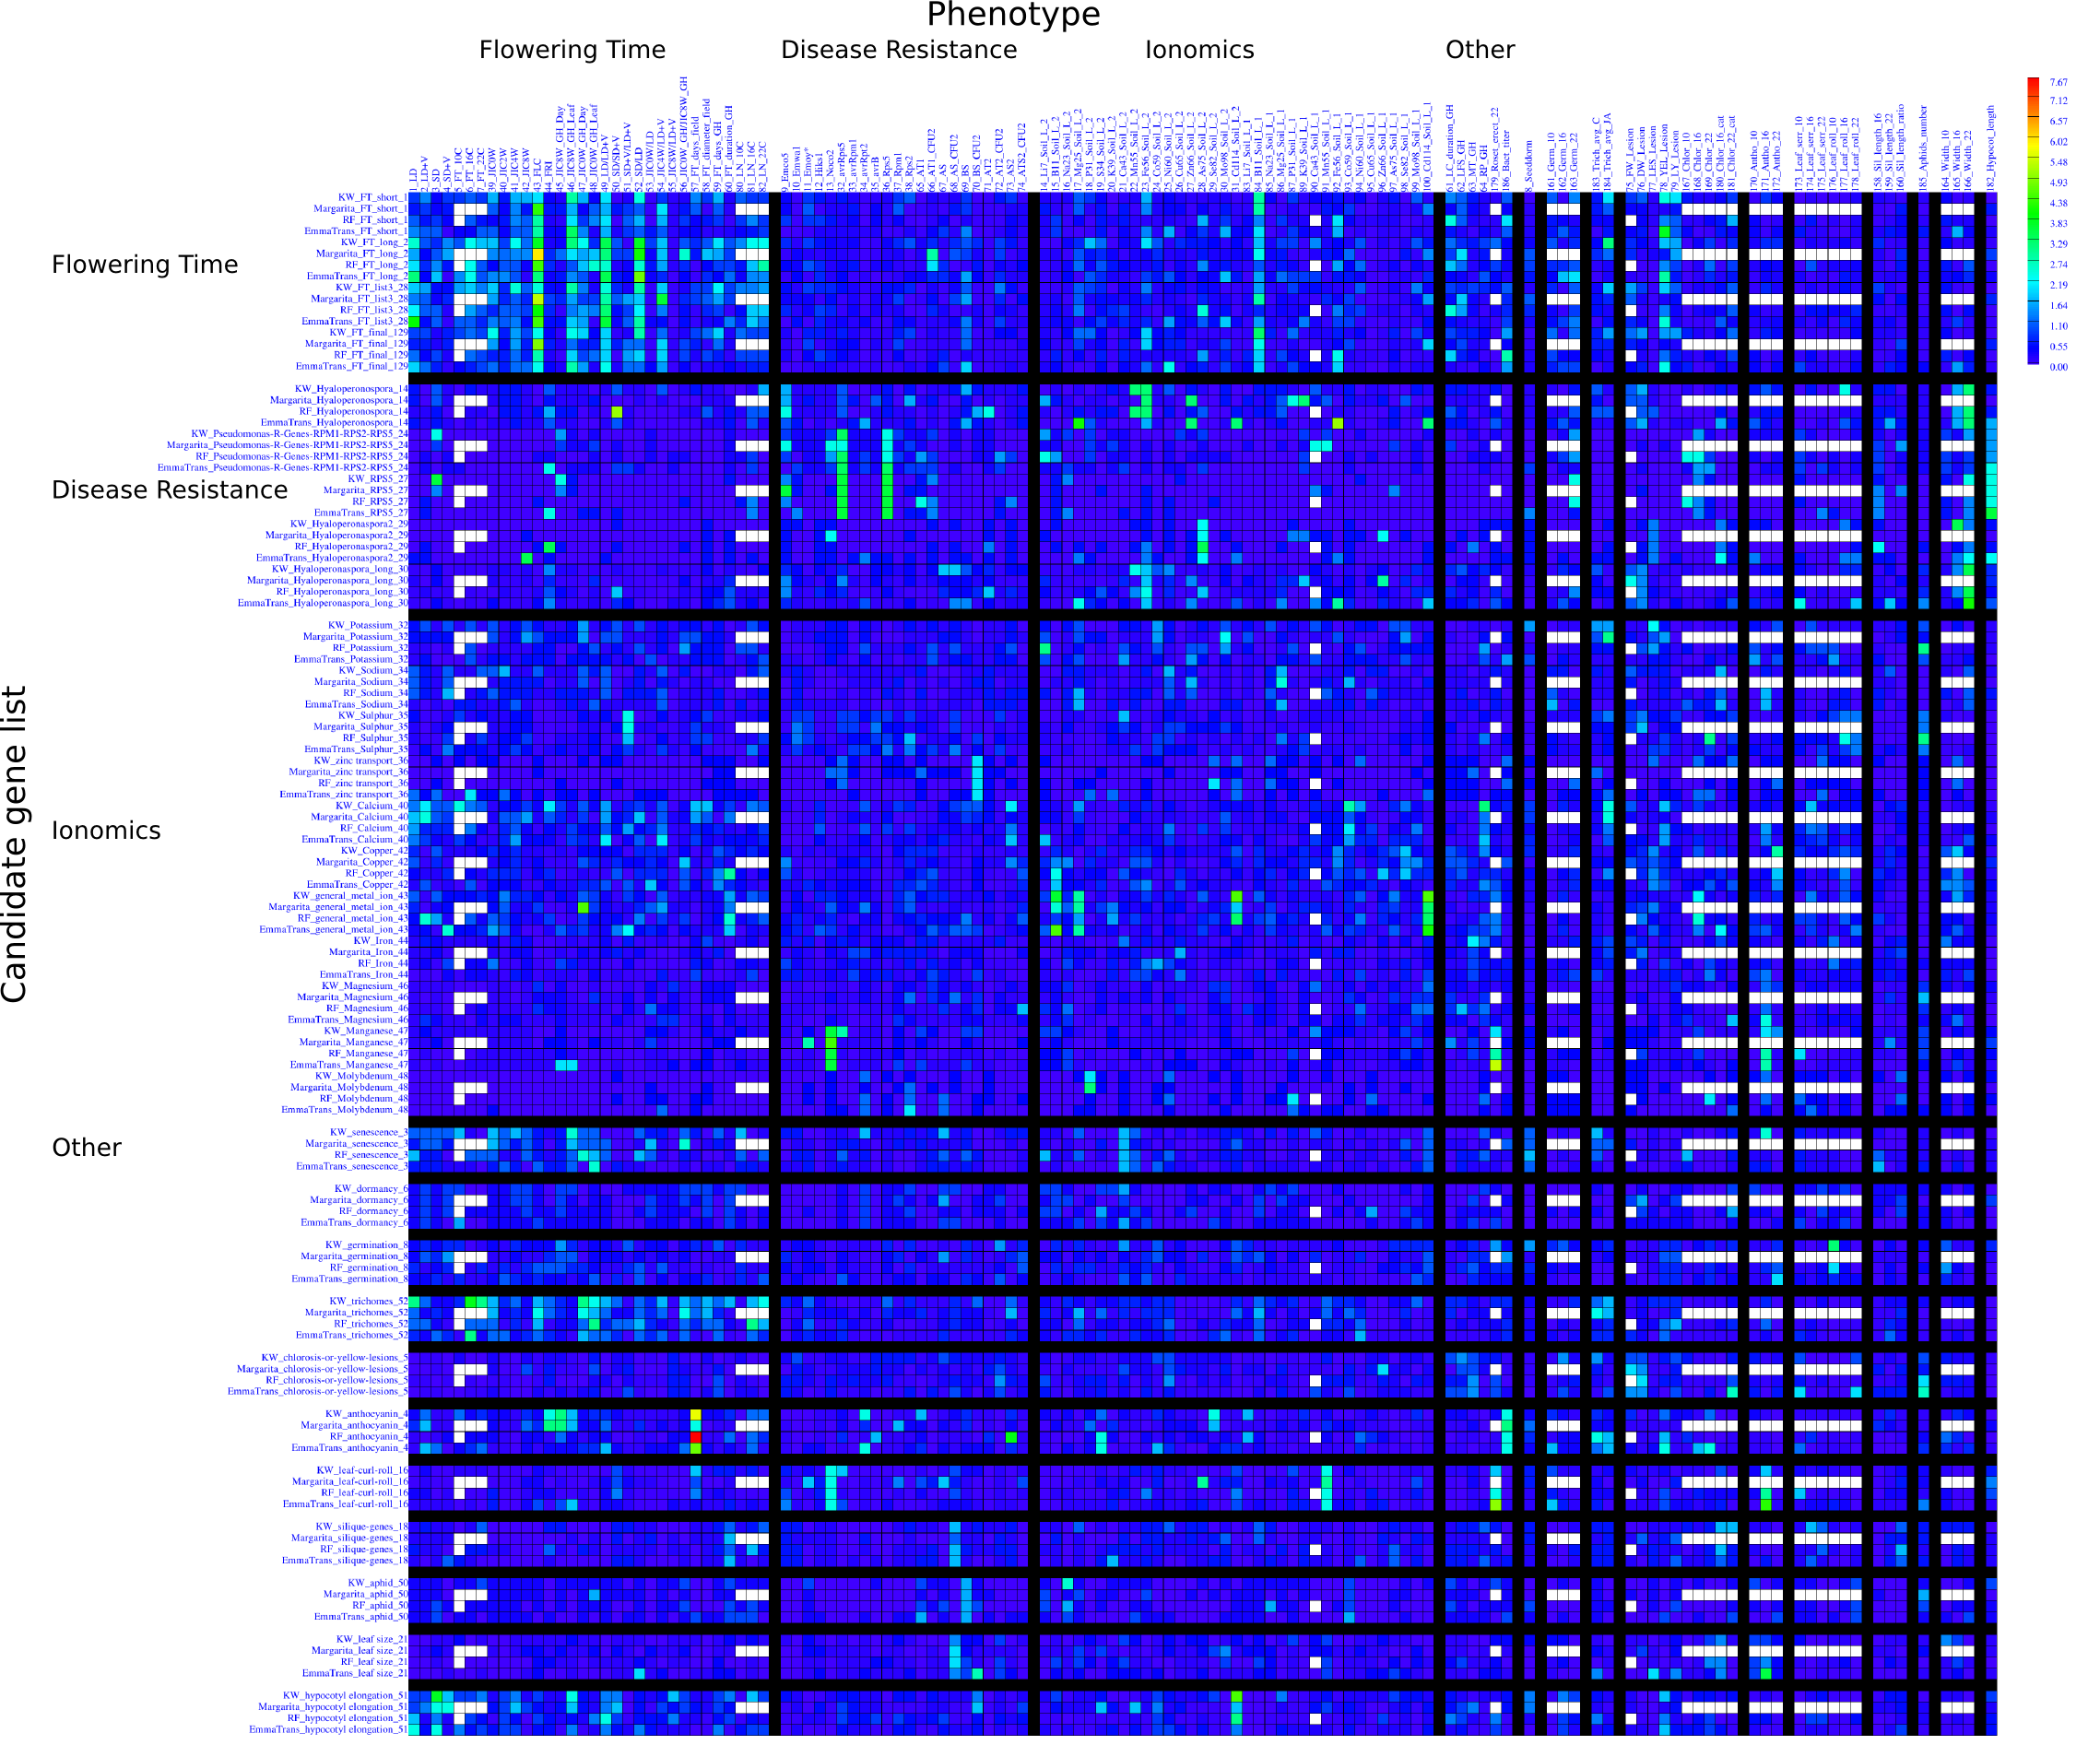
\includegraphics[width=1\textwidth]{figures/top_snp_test_call_method_17_f1000_m20000_inkscape.png}
  \caption{Enrichment of candidate genes among top 1000 genes. All genes within 20,000 bp from the SNP are assigned with that SNP's pvalue. In case of one gene having multiple pvalues from different SNPs, the maximum will be taken as that gene's pvalue. Rows are different types of candidate gene list with different methods. Columns are different phenotypes. Black bar separates similar groups of phenotypes.}\label{f5}
\end{figure}

\subsection{Overlapping top-ranked genes of results from different phenotypes}
Apart from whether one result shows enrichment for a particular candidate gene list, we also checked whether results from similar phenotypes have similar genes on top, or two results from distinct phenotypes, both showing enrichment for a particular candidate gene list, are picking same group of genes on the top, Figure~\ref{f6}. This is a much more specific figure compared to the candidate gene enrichment one, Figure~\ref{f3}. This confirms each priori candidate gene list is quite diversified, which causes the same candidate gene list significant in several phenotypes. Signal in flowering time phenotype is very strong even when top 1000 ranked genes are pulled in, Figure~\ref{f7}.

\begin{figure}
  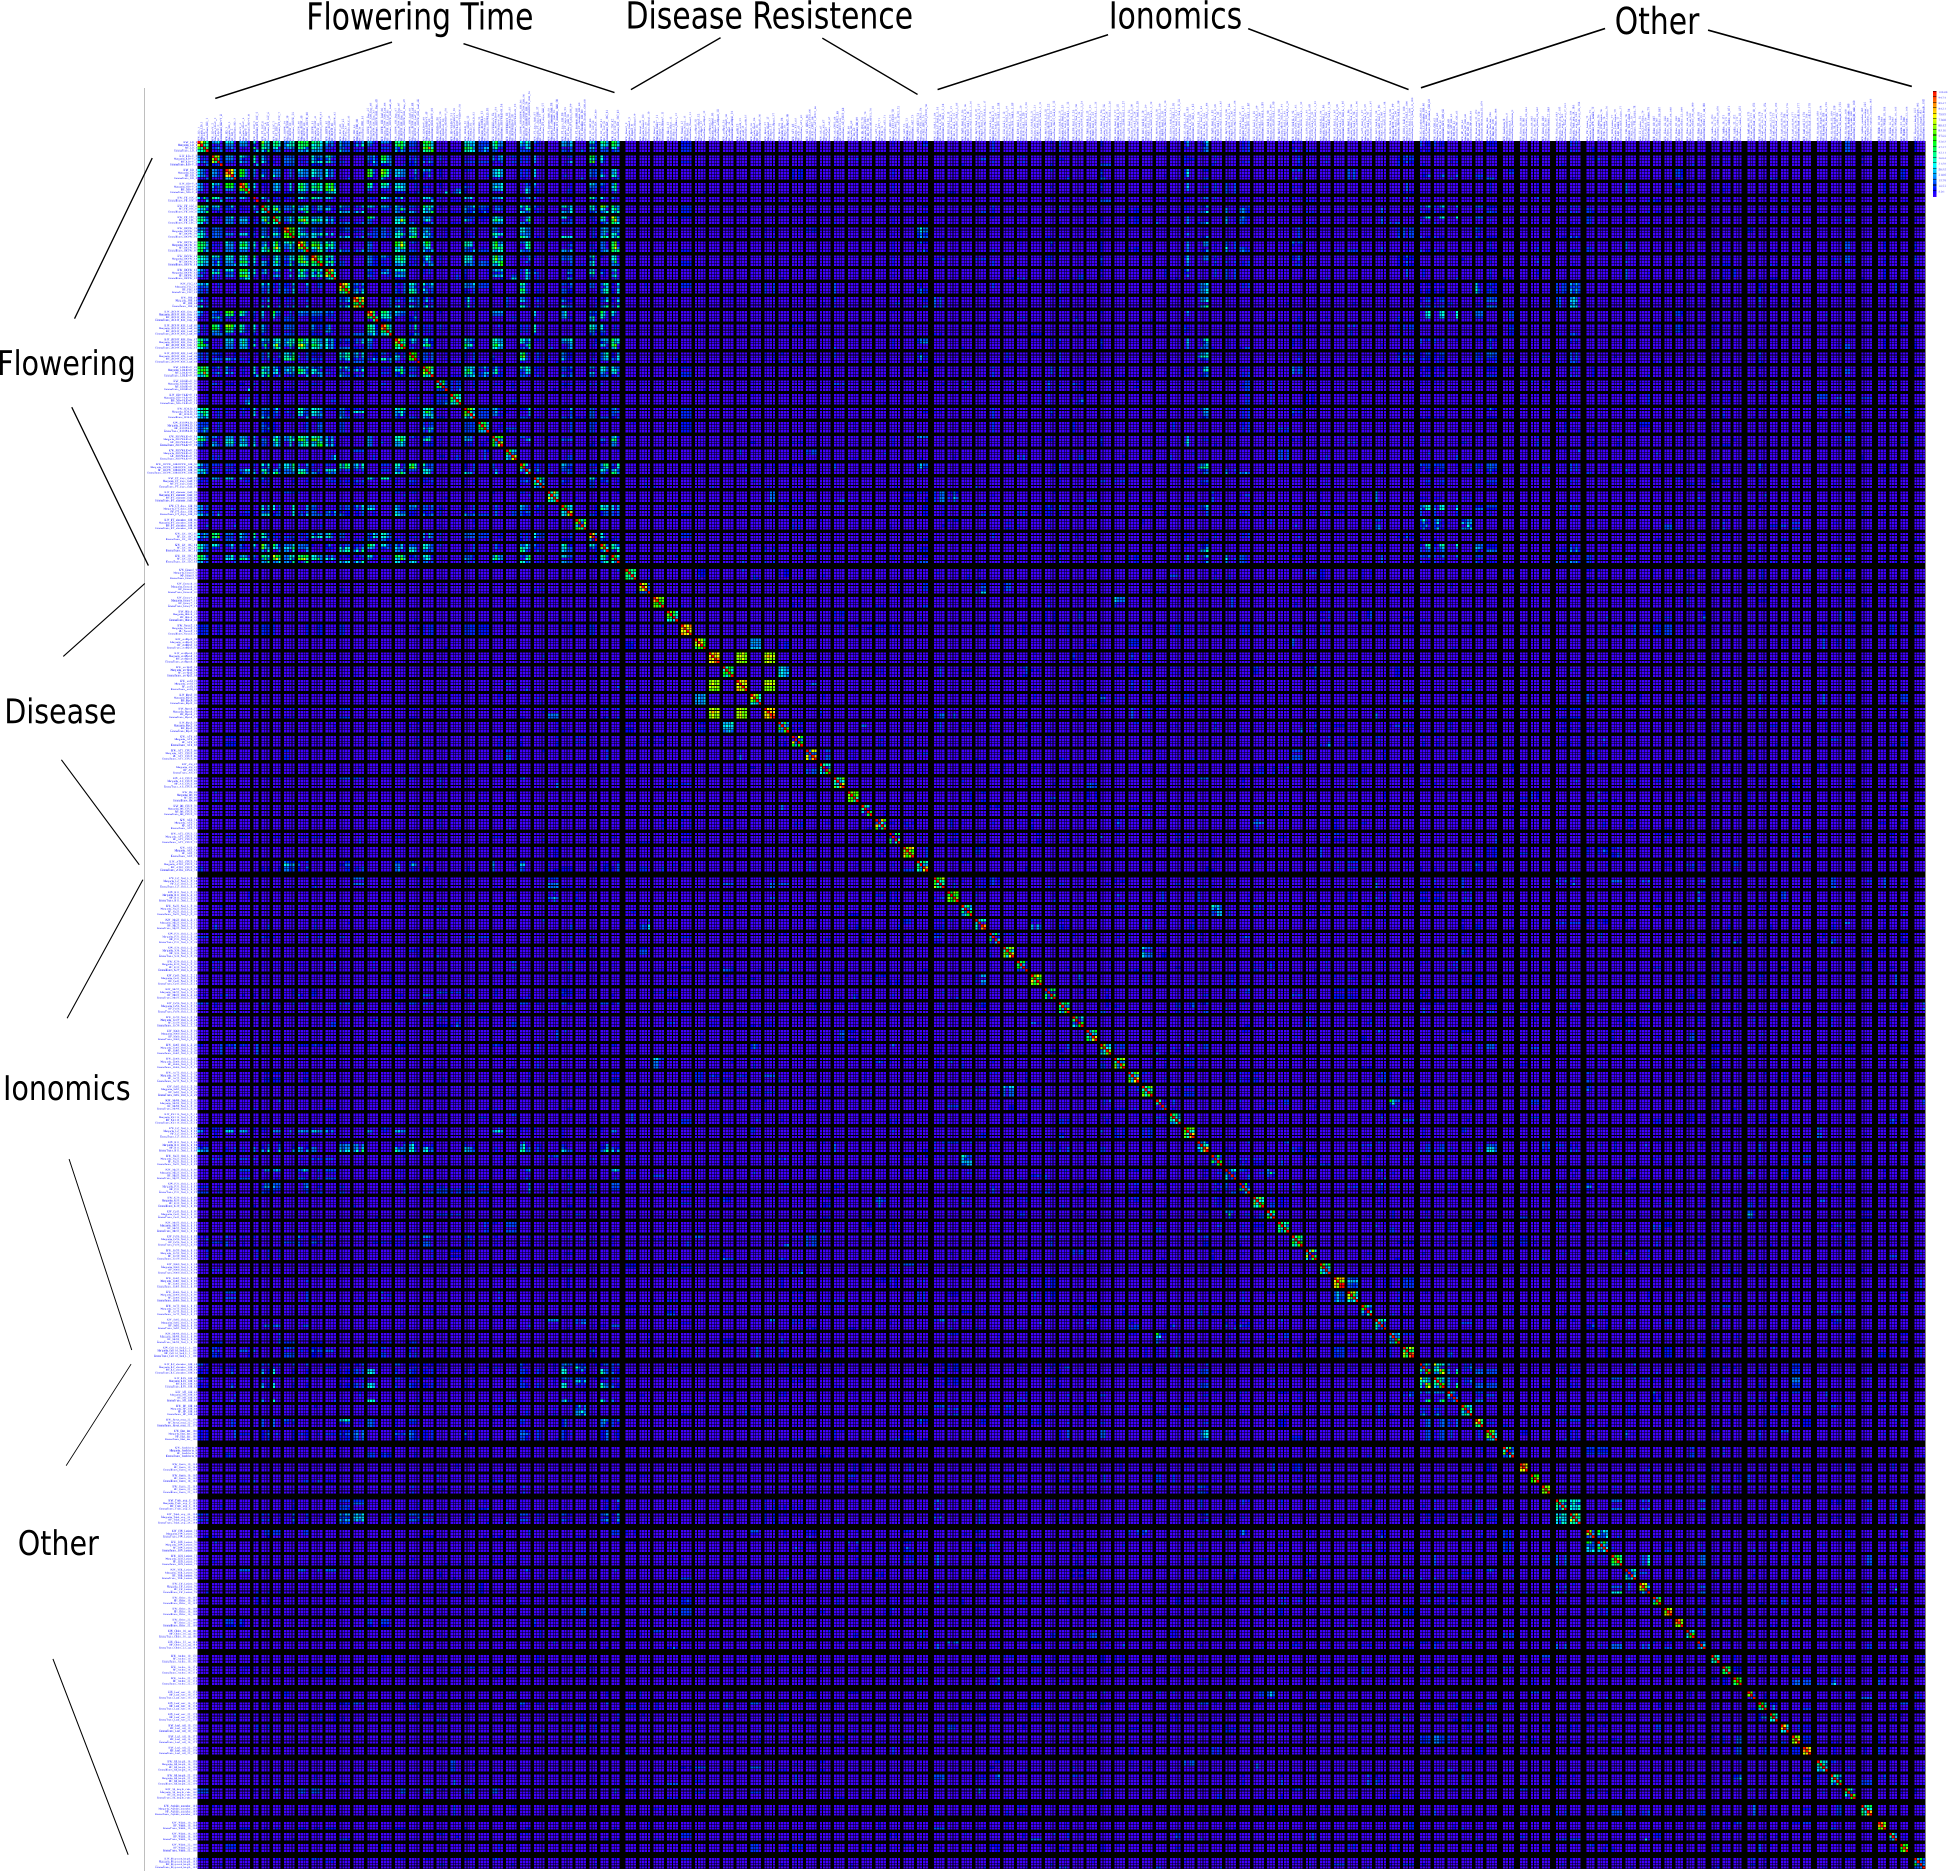
\includegraphics[width=1\textwidth]{figures/overlapping_results_a100_inkscape.png}
  \caption{Overlapping of top 100 genes. All genes within 20,000 bp from the SNP are assigned with that SNP's pvalue. In case of one gene having multiple pvalues from different SNPs, the maximum will be taken as that gene's pvalue. Rows and columns are same, results from different phenotypes. Thick black bars separate similar groups of phenotypes. Slender black bars separate different phentoypes.}\label{f6}
\end{figure}

\begin{figure}
  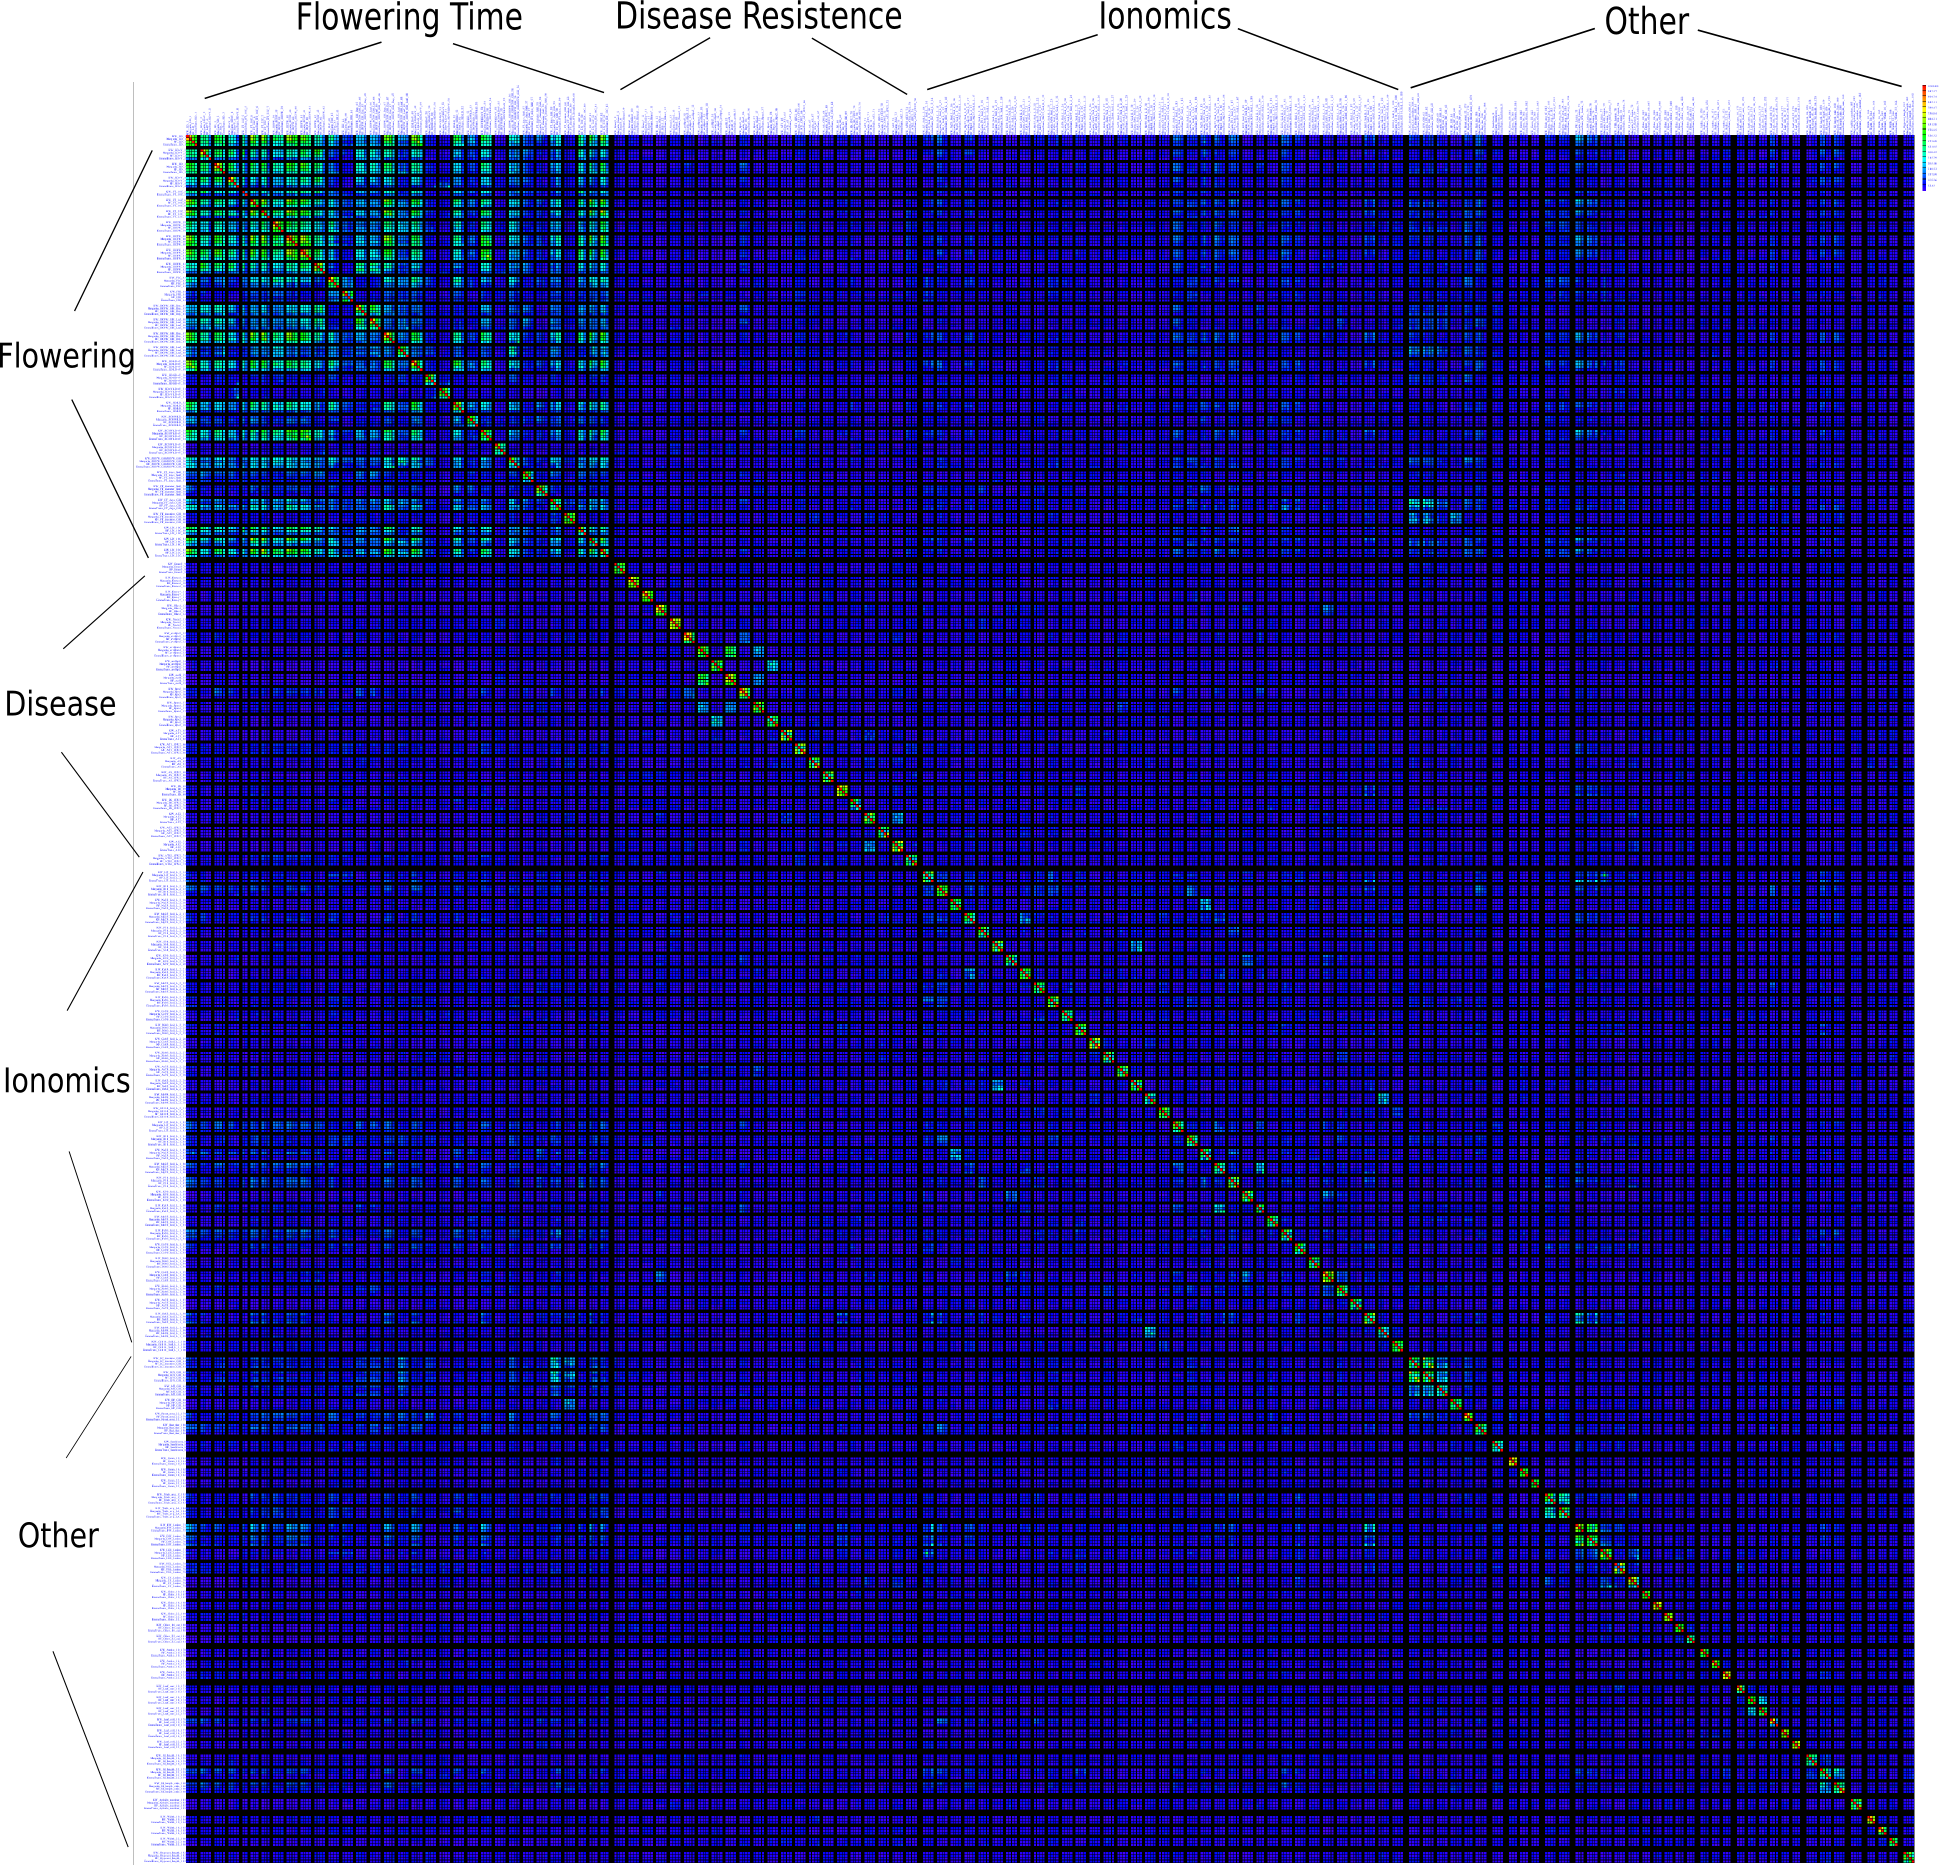
\includegraphics[width=1\textwidth]{figures/overlapping_results_a1000_inkscape.png}
  \caption{Overlapping of top \textbf{1000} genes. All genes within 20,000 bp from the SNP are assigned with that SNP's pvalue. In case of one gene having multiple pvalues from different SNPs, the maximum will be taken as that gene's pvalue. Rows and columns are same, results from different phenotypes. Thick black bars separate similar groups of phenotypes. Slender black bars separate different phentoypes.}\label{f7}
\end{figure}

\section{Detailed example}

Gene FLC is well captured in Figure~\ref{f8}. The region contains the \textbf{second-highest} peak in results from Emma. LD is very messy in this region, echoing strange haplotype structured observed in previous papers.

\begin{figure}
  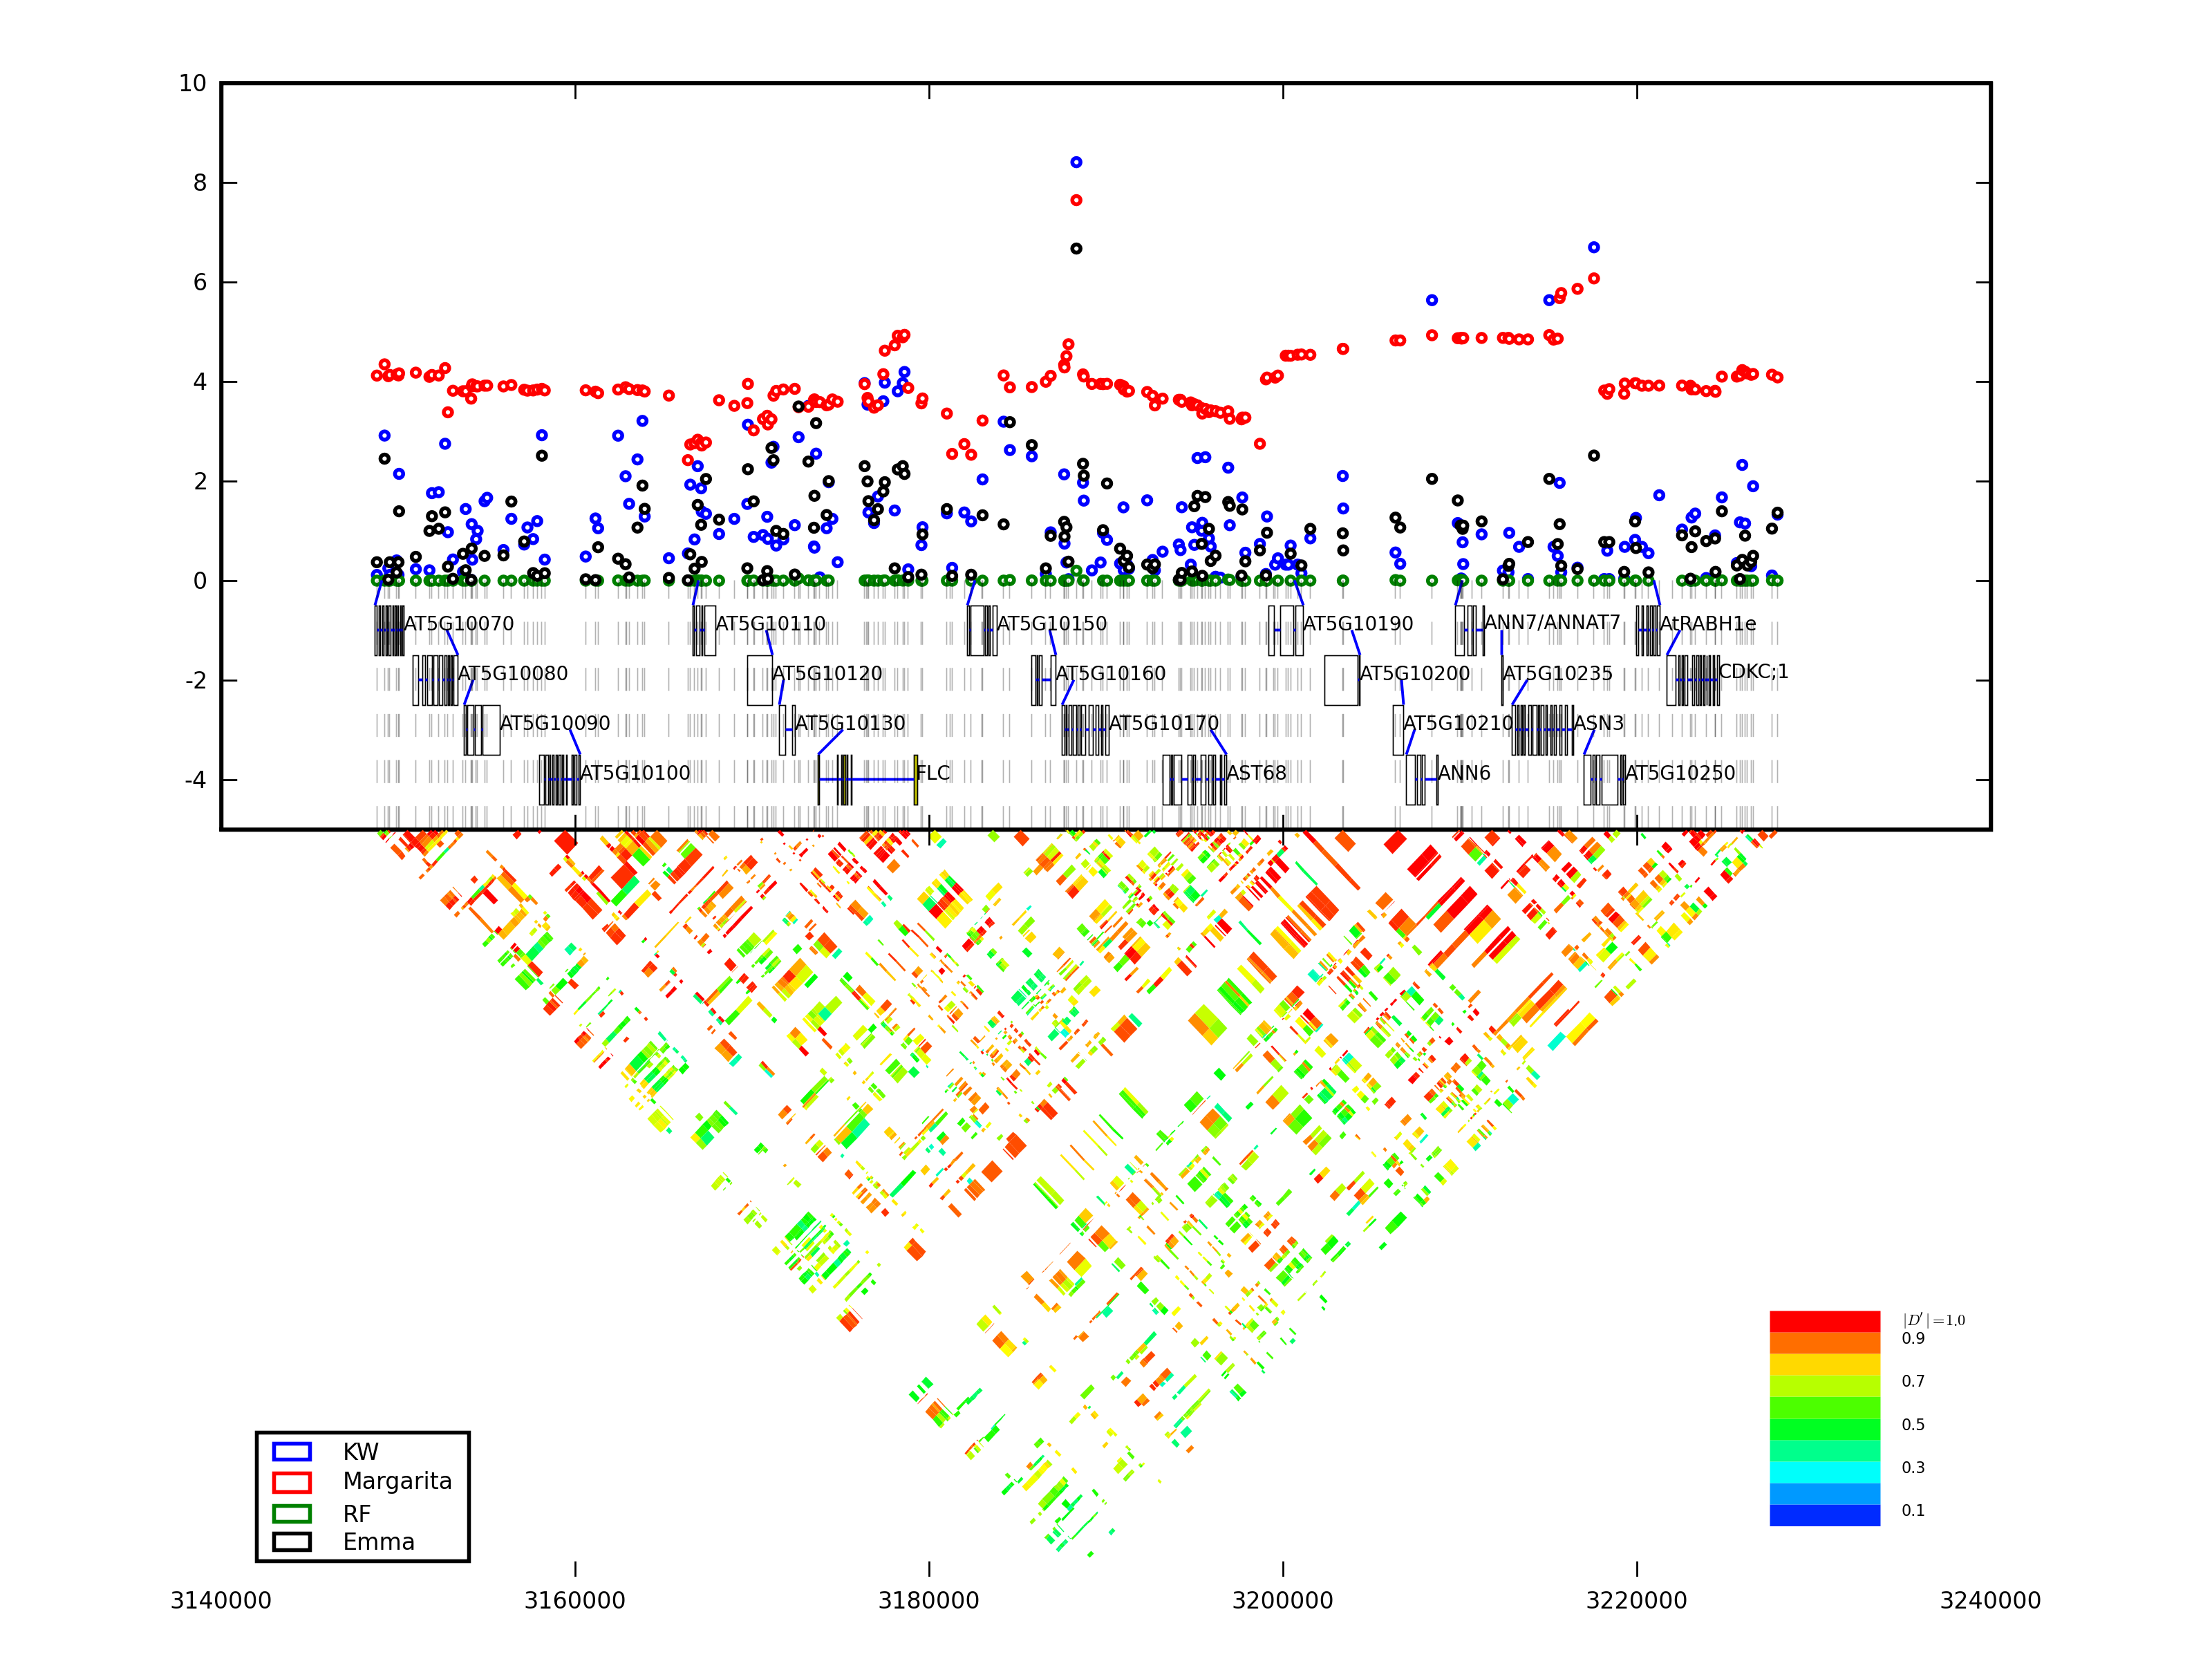
\includegraphics[width=1\textwidth]{figures/phenotype_1_LD_rank_12_snp_5_3188328_list_type_28_FT_list3_gene_830876_AT5G10120.png}
  \caption{X-axis is chromosomal position (chromsome 5). Y-axis is minus log(pvalue). Phenotype is long-day flowering time. Scores of Margarita and RandomForest(RF) are normalized against Kruskal-Wallis pvalues. Lower panel displays LD in this 80kb region. Exons of FLC are colored in yellow.}\label{f8}
\end{figure}




\bibliography{gwa}
\bibliographystyle{apalike}

\end{document}
